\title{ \vspace{5cm}
\begin{Huge}
\textsc{Algorithms and Computability
Project Report}\\ 
\end{Huge}
\begin{Large}
\textsc{The 2D Bin Packing Problem}
\end{Large}
\vspace{1cm}}
\author{
Igor Sa\l uch\\
Jianhao Luo
}
\date{}

\documentclass[12pt]{article}
\usepackage[margin=1in]{geometry}
\usepackage{graphicx}
\graphicspath{ {img/} }
\usepackage{float}
\usepackage{csquotes}
\usepackage{hyperref}
\usepackage{listings}
\usepackage{xcolor}
 
\definecolor{codegreen}{rgb}{0,0.6,0}
\definecolor{codegray}{rgb}{0.5,0.5,0.5}
\definecolor{codepurple}{rgb}{0.58,0,0.82}
\definecolor{backcolour}{rgb}{0.95,0.95,0.92}
 
\lstdefinestyle{mystyle}{
    backgroundcolor=\color{backcolour},   
    commentstyle=\color{codegreen},
    keywordstyle=\color{magenta},
    numberstyle=\tiny\color{codegray},
    stringstyle=\color{codepurple},
    basicstyle=\ttfamily\footnotesize,
    breakatwhitespace=false,         
    breaklines=true,                 
    captionpos=b,                    
    keepspaces=true,                 
    numbers=left,                    
    numbersep=5pt,                  
    showspaces=false,                
    showstringspaces=false,
    showtabs=false,                  
    tabsize=2
}
 
\lstset{style=mystyle}
\begin{document}
\begin{titlepage}
\maketitle
\vfill
{\centering \large November 19, 2019 \par}
\pagenumbering{gobble}
\end{titlepage}
\newpage
\pagenumbering{arabic}


\section{Introduction}
It is a common problem of trying to pack a lot of items in limited space.
For example, truck loaders deal with such problem every day --
how to load a truck as efficiently as possible,
but without overloading the vehicle.
It is also sometimes called ``a thief problem'', where a burglar tries
to pack as many items as possible into their backpack.

In computer science, we also deal with this problem very often.
Packing virtual machines on a server with limited memory is a problem set
on completely different kind of resources,
but still solved using the same principles.
For example, we want to present the user their photos on the thumbnail view,
without cropping, while retaining the sizes (or at least ratios).

\section{Problem description}
The bin packing problem,
is an combinational optimization problem. % TODO ensure
According to Wikipedia\cite{wikibinpacking},
\begin{displayquote}
\textelp{} items of different volumes must be packed into a finite number of
bins or containers each of a fixed given volume in a way that minimizes the
number of bins used.
\end{displayquote}
The problem has many variations,
it arises in various places where space resources are limited and there is a
need to find the best packing.

In our case, the limited resource is a \textbf{two dimensional space}.
We have a set of rectangles (blocks),
each with its own \textbf{height} and \textbf{width}.
In addition, each block has it's own \textbf{value}.
We want to score as much value points as we can,
by fitting in a fixed space as much blocks (of the best values),
as we can.

\section{Solution}
\subsection{Solution description}
Before diving into details, let us start with a brief,
step-by-step description of the algorithm.

\begin{enumerate}
  \item For each permutation of the input set, do the following:
  \begin{enumerate}
    \item Put the first item from the list in the top left corner,
    \item Split the remaining space into 2 rectangles, one on the right
      to the first item, another below,
    \item Repeat steps 2 and 3 recursively in the form of a binary tree
      until there is no more space left.
    \item Save the value score.
  \end{enumerate}
  \item Compare scores and pick the best packing. 
\end{enumerate}

\subsubsection{Permutation}
First we permutate our input set in order to get all possible packings.
Then we can proceed to find the best fit for each permutation.

\subsubsection{Placing the block}
This step is quite simple -- we need to put the block somewhere,
and one of the corners would let us have a two-rectangle split for the next step.
Top left corner is an arbitrary choice -- it can be any other corner as long
as we are consistent with our choice.
We store all whitespace rectangles in a binary tree.

\subsubsection{Splitting the remaining space}
We divide the remaining whitespace in order to allow recursion.
Each smaller part can be treated as a new rectangle
for fitting blocks from our queue.
\begin{figure}[H]
  \centering
	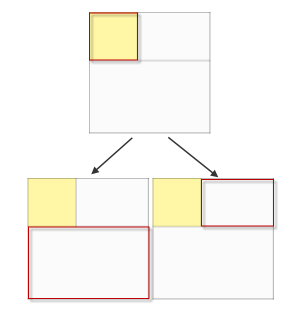
\includegraphics[width=.5\textwidth]{split}
  \caption{Visualisation of splitting the space and binary tree creation}
  \label{fig:split}
\end{figure}

\subsubsection{Recursion}
Finally, we do the same thing again for each new item to pack,
and for the each smaller whitespace rectangle.
There is one caveat, though -- we do it in a form of binary tree.
It simply means that we traverse our tree to find the smallest free space
in which our rectangle would fit.
If there is no such space, we discard our block and proceed to the next one.

\subsubsection{Saving and comparing scores}
After calculating all packings for each permutation,
we can pick one of the best value.

\subsection{Solution pseudocode}
\begin{lstlisting}[language=Python, caption=Python-style pseudocode]
class Rectangle:
    left: int
    right: int
    top: int
    bottom: int
    value: int

current_score: int = 0

class Node:
    child_node[2]: Node
    space: Rectangle  # free space rectangle
    blockid: int

    def insert(block: Rectangle):
      if we are not a leaf:
          # try inserting into first child
          new_node = child_node[0].insert(block)
          if new_node != None:
              return new_node
          # else there is no room, insert into the second child
          return child_node[1].insert(block)
      else:
          # if there is already a block here
          if self.blockid != None:
              return None
          if block does not fit in self.space:
              return None
          if block fits perfectly in self.space:
              return self
          # otherwise, split this node and create children
          current_score += block.value
          self.child_node[0] = Node()
          self.child_node[1] = Node()

          # decide which way to split
          dw = space.width - block.width
          dh = space.height - block.height

          if dw > dh then:
            child_node[0].space = (
              space.left,
              space.top,
              space.left + block.width - 1,
              space.bottom,
            )
            child_node[1].space = (
              space.left + block.width,
              space.top,
              space.right,
              space.bottom,
            )

          else:
            child_node[0].space = (
              space.left,
              space.top,
              space.right,
              space.top + block.height - 1,
            )
            child_node[1].space = (
              space.left,
              space.top + block.height,
              space.right,
              space.bottom,
            )

          # insert into first child we created
          return self.child_node[0].insert(block)

def find_best(input: Rectangle[]):
  for each permutation[i] of input:
    root[i] = Node()
    for each block in input:
      # insert the next block
      root[i].insert(block)
    # save and reset score
    score[i] = current_score
    current_score = 0
  best_score = max(score)
  best_score_index = max_index(score)
  return root[best_score_index], best_score
\end{lstlisting}

\subsection{Pseudocode description}
The \texttt{Node.insert} function traverses the tree looking for a place
to insert the block.
It returns the node the block can be placed into or \texttt{None} to say
it could not fit.

The code that calls \texttt{Node.insert} can then use the rectangle
from the returned node to figure out where to place the block in the space,
then update the node's \texttt{block\_id} to use as a handle for future use.

\subsection{Solution correctness proof}
% TODO

\section{Conclusion}
% TODO

\newpage
\begin{thebibliography}{9}
\bibitem{wikibinpacking}
	\url{https://en.wikipedia.org/wiki/Bin_packing_problem}
\end{thebibliography}

\end{document}
